% Created 2024-09-02 Mon 23:34
% Intended LaTeX compiler: pdflatex
\documentclass[letterpaper, 12pt]{article}
\usepackage[utf8]{inputenc}
\usepackage[T1]{fontenc}
\usepackage{graphicx}
\usepackage{longtable}
\usepackage{wrapfig}
\usepackage{rotating}
\usepackage[normalem]{ulem}
\usepackage{amsmath}
\usepackage{amssymb}
\usepackage{capt-of}
\usepackage{hyperref}
\usepackage{minted}
\usepackage{xcolor}
\usepackage{hyperref}
\usepackage{tocloft}
\usepackage{minted}
\usemintedstyle{manni}
\usepackage{pdfpages}
\usepackage{fancyhdr}
\usepackage{graphicx}
\usepackage[top=1.4in, left=0.5in, right=0.5in, bottom=0.8in]{geometry}
\usepackage[T1]{fontenc}
\usepackage{helvet}
\pagestyle{fancy}
\renewcommand{\headrulewidth}{0pt}
\renewcommand{\footrulewidth}{0pt}
\setlength{\parindent}{0em}
\setlength{\parskip}{1em}
\usepackage{hyperref}
\usepackage {color}
\usepackage {tabularray}
\usepackage{xcolor}
\hypersetup{
colorlinks=true,
linkcolor=blue,
filecolor=magenta,
urlcolor=cyan,
citecolor=green,
pdfborder={0 0 0}
}
\usepackage[most]{tcolorbox}
\author{Hilduara Abreu}
\date{2024-09-05}
\title{PS 192 | Missing Student Protocol SY 2024-25\\\medskip
\large Implementation of the Missing Student Protocol, effective September 5th, 2024}
\hypersetup{
 pdfauthor={Hilduara Abreu},
 pdftitle={PS 192 | Missing Student Protocol SY 2024-25},
 pdfkeywords={},
 pdfsubject={},
 pdfcreator={Emacs 29.4 (Org mode 9.6.15)}, 
 pdflang={English}}
\begin{document}

\fancyfoot[C]{\setlength{\unitlength}{1in}\begin{picture}(5,0)\put(-1.8,-0.5){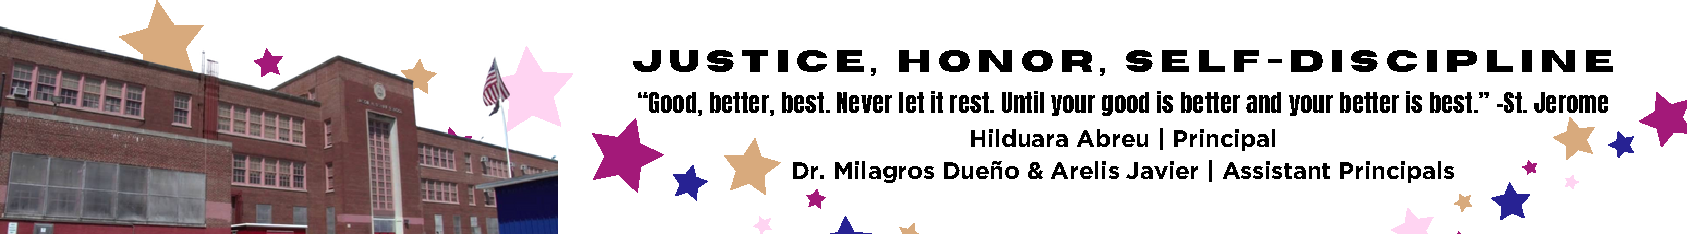
\includegraphics[width=8.8in,height=1.3in]{logo-1}}\end{picture}}
\fancyhead[C]{\setlength{\unitlength}{1in}\begin{picture}(5,0)\put(-1.9,-0.5){
\includegraphics[width=8.9in,height=1.3in]{logo-2}}\end{picture}}
\fancyhead[R]{\thepage}
\pagenumbering{gobble}

\begin{document}
\newpage
\vspace*{-0.5cm}

\textbf{Implementation of the Missing Student Protocol, effective September 5th, 2024}

\textbf{Purpose}

The safety and well-being of our students are of the utmost importance at PS 192. This Missing Student Protocol outlines the immediate actions required when a student is identified as missing, ensuring a swift, efficient, and legally sound response by all staff members. This protocol aligns with the New York City Department of Education (NYC DOE) regulations and is designed to provide clarity, consistency, and accountability in handling such critical situations.

\textbf{Reporting a Missing Child}
\begin{itemize}
\item Immediate Reporting: If a staff member identifies a missing child, they must immediately use their cell phone to text Assistant Principal, Dr. Dueno, and Parent Coordinator Ms. Rijo, while actively searching for the child.

\item Building Response Team (BRT) Activation: Upon confirmation that a child is missing, the Principal will activate the Building Response Team (BRT) to assist in locating the student and preventing them from leaving the premises.
\end{itemize}

\textbf{Search Efforts}
\begin{itemize}
\item Comprehensive Search: The BRT, along with all available school staff, will conduct a thorough search of both indoor and outdoor areas across the entire school premises.
\item Parent/Guardian Contact: A member of the administration team will immediately contact the parent or guardian to confirm possible early pick up by the parent or guardian designee.
\item Intercom Announcement: An announcement will be made via the school-wide intercom by the secretary, using the code phrase: "The lion is out of the den. Call me if you see him or find him." This alert serves to notify all staff of the missing child and to gather information regarding the student’s last known location.
\item Law Enforcement Notification: If the child is not found within a predetermined time frame (typically 5-10 minutes), local law enforcement will be notified immediately. The Principal and/or the BRT chairperson will be responsible for contacting 911, as well as informing the Borough Safety Director and the District 6 (D6) Superintendent. Upon law enforcement's arrival, the Principal and/or BRT chairperson will provide a comprehensive student information profile, including recent photos, known locations, and any other relevant details.
\end{itemize}

\textbf{Communication, Documentation, and Feedback}
\newpage \vspace*{-0.5cm}
\begin{itemize}
\item \textbf{Parent/Guardian Notification:} A member of the administration will immediately contact the parent or guardian to inform them of the situation, providing timely updates as the situation develops.
\item Incident Documentation: The staff members responsible for the child's supervision at the time of the incident must complete an Online Occurrence Reporting System (OORS) report detailing the incident before leaving the premises. This report must be submitted to Assistant Principal Dr. Milagros Dueño. The OORS report must be filed within 24 hours by either Dr. Dueño or Ms. Javier.
\item \textbf{Incident Review}: The Principal, in collaboration with the UFT Chapter Leader and the BRT chairperson, will review the incident report. Feedback will be gathered from all involved parties. Based on the data collected and the feedback provided, the Principal may convene a disciplinary meeting with the involved staff members if any procedural lapses are identified.
\end{itemize}

\textbf{Preventive Measures}
\begin{itemize}
\item \textbf{Diligent Supervision}: When a child or group of students is assigned to a staff member, that staff member is responsible for the safety and well-being of the student or students for the duration of the service they are providing.
\item \textbf{Hallway and Bathroom Monitoring}
\begin{itemize}
\item \textbf{Second Floor:} Ms. Del Orbe, Ms. Cuesta, and Mr. Suero are responsible for monitoring the second-floor hallway and bathrooms.
\item \textbf{First Floor:} Ms. Clemons, Ms. Rijo, and the designee assigned by the Principal of MS 209 are responsible for supervising the first-floor hallway and bathroom facilities.
\end{itemize}
\item \textbf{Doors and Alarm Inspection}: Ms. Clemons, our School Safety Agent, will conduct frequent inspections of alarms and ensure all exits are secured to prevent unauthorized egress or access.
\item Signage and Alarm Management: Signs will be placed on exits used for arrival and/or dismissal, specifying times when the alarm will be deactivated. Assigned personnel are responsible for deactivating and reactivating the alarm during these times.
\item Student Safety Education During the SEL (Social-Emotional Learning) block, teachers will educate students on safety procedures and provide guidance on whom to contact if they feel lost or unsafe. This education will occur monthly.
\end{itemize}

Your cooperation and strict adherence to this protocol and the preventive measures outlined are crucial to ensuring the safety and security of our students. By working together and maintaining vigilance, we can \newpage \vspace*{-0.5cm}
 significantly contribute to the overall safety of our school environment.

We thank you for your attention to this matter and your commitment to the safety and well-being of our students.

With Justice, Honor, and Self-Discipline,


\includegraphics[width=0.2\textwidth]{hil_signature}

\textbf{Hilduara Abreu, Principal}

\textbf{The school of Joyful Learning!}

\href{www.ps192.org}{www.ps192.org}
\end{document}
